\documentclass[oneside,12pt]{amsart}
\usepackage[english]{babel}
\usepackage{graphicx}
\usepackage{float}
\usepackage{mathtools}
\usepackage{amsfonts}
\usepackage{amssymb}
\usepackage{siunitx}
\usepackage{amsthm}
\usepackage{enumitem}
\usepackage{stmaryrd}
\usepackage{multirow}
\usepackage[backend=bibtex,style=numeric]{biblatex}
\bibliography{Biblio}
\usepackage[a4paper, total={6in, 10in}]{geometry}
\graphicspath{{./}{}}% You can add the path for the images in the empty brackets 
\title{Study of Electrostatics: Generation and Measurement of Charge}
\author{Josh Goldfaden, Daniel Briseno}
\date{}
\newdimen\graph
\graph=4.2in
\newdimen\medgraph
\medgraph = 5.3in
\newdimen\smallgraph
\smallgraph = 3in
\newdimen\tinygraph
\tinygraph = 1.5in
\renewcommand{\arraystretch}{1.5}
\begin{document}
	\section{Abstract}
	In this series of experiments, Coulomb’s law was evaluated experimentally through first charging a top (T) strip of tape and a bottom (B) strip of tape and analyzing their interactions. In particular it was observed that (insert observations). Further, a virtual lab was conducted in which a hanging sphere was suspended, and its force body diagram was diagrammed and analyzed. Further, this sphere is placed in close proximity to a neighboring sphere attached to a rod, and their interactions were studied, specifically the magnitude of the Coulomb's force the suspended ball experienced was computed. It was found that (insert findings). One final virtual analysis that simulated the interaction between a suspended ball and the center of a charged rod. In this experiment, it was determined that (insert findings). In the final portion of the lab, Coulomb’s law was used to determine the discharge rate of a series of a virtual series of suspended spheres. 
	\section{Introduction}
	One experimental law of physics that is fundamental in understanding electrostatic forces is Coulomb’s law: 
	\begin{align}
		|\vec{F}^E_{12}| &= k_e \frac{|q_1 q_2|}{r_{12}^2}\\
		\vec{F}^E_{12} &= k_e \frac{|q_1 q_2|}{r_{12}^2} \hat{r}_{12} 
	\end{align}
	
	\indent This mathematical rule states that the magnitude of the force is the product of two charged particles, designated as $q_1$ and $q_2$ in units of Coulombs (unit of charge), and Coulomb’s constant (designated as $k_e$ with the unit N$\text{m}^2$/$\text{C}^2$) divided by the distance between the two particles squared, which is designated as $r_{12}$ with the unit $\text{m}^2$. It is noteworthy that Coulomb’s constant is a proportionality constant that relates different electric variables.\\ 
	
	\indent With respect to the implications of Coulomb’s law, in this particular lab, the electrostatic force exerted by a virtual charged sphere suspended by a rope  on a neighboring, virtual charged sphere attached to a rod. It is noteworthy that the sphere suspended by the rope is held at one 
	\section{Electric Field Due to a Line of Charge}
	\indent In this virtual lab, we wanted to measure the electrostatic force a charged rod exerts on a hanging test charge. (a hanging charged sphere). In order to measure the electric field strength created by the rod at different radii, we hanged a ball with 35nC of charge and measured how much the ball was displaced when a charged rod of length 0.7104m was brought near it. Given the displacement of the ball and the ball's mass, we were able to determine the electric force acting on the ball. Given the charge of the ball, we were able to determine what the electric field magnitude due to the rod at the position of the ball. The results of our measurements are shown in Figure 1.\\
	
	\begin{figure}[h]
		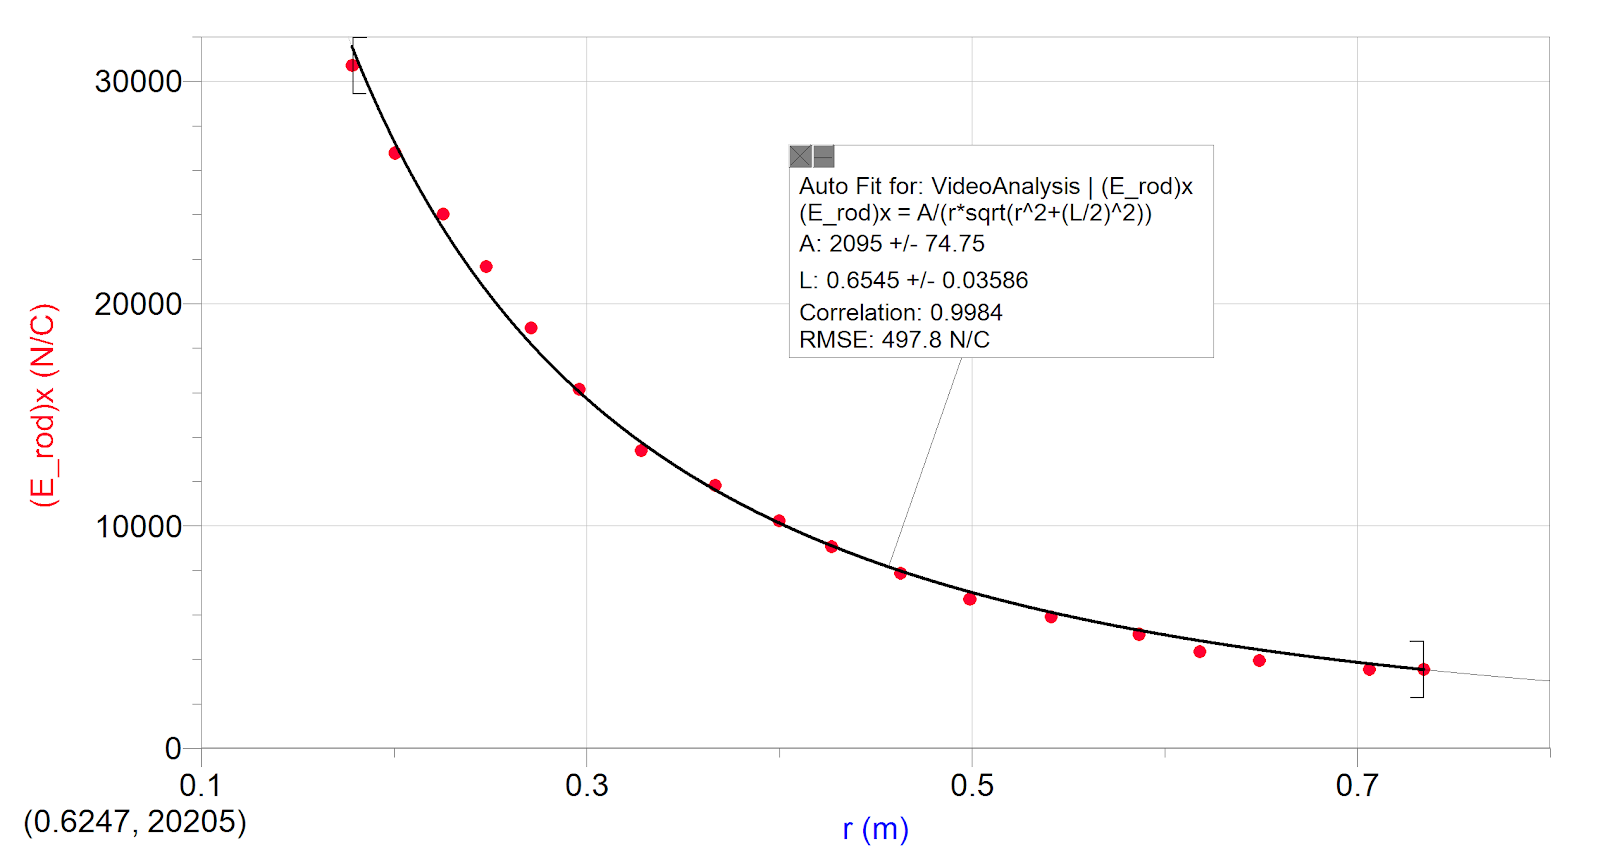
\includegraphics[width=\medgraph,scale=0.01]{FieldStrength.png}
		%h (here) - same location
		%t (top) - top of page
		%b (bottom) - bottom of page
		%p (page) - on an extra page5
		%! (override) - will force the specified location
		\caption{The electric field of the virtual rod (N/C) plotted against its distance from the charged sphere (m). 
		}
		\label{Fld}
	\end{figure}
	
	\indent Note that the line of best fit is given by :
	\begin{align*}
	x=\frac{A}{r\sqrt{r^2+(L/2)^2}	}
	\end{align*}
	where $A\approx 2095$, L is the length of the rod and r is the distance between the rod and the ball.
	
	\indent We are given that $A\approx kQ_{rod}$. From this we can derive the charge present on the rod. We predict that the rod will likely have a charge magnitude that is significantly greater than the hanging charge, since we obtained charges greater than 35nC by friction in previous experiments. To obtain the exact value of the charge on the rod, we compute:\\
	\begin{align*}
	2095\:\text{Nm}^2/C &\approx kQ_{rod}\\
	\frac{2095\:\text{Nm}^2/C}{k}&\approx Q_{rod}\\
	Q_{rod}&\approx 0.233\mu\text{C}
	\end{align*}
	
	\indent And indeed we see that $Q_{rod}>Q_{ball}$. We would also like a mathematical derivation of the equation for the line of best fit, so that we may better understand the electric field generated by a thin rod.\\
	
	\indent Since we only know how to derive the electric field generated by a point-particle, we orient the rod such that it lies on the y-axis on an x-y plain and then divide the rod into infinitesimally small pieces of length $dy$, such that each piece acts like a point-particle. Then, the charge of that particle would be $dy\cdot \lambda$, where $\lambda = Q_{rod}/L$ is the charge density of the rod.\\
	
	\indent With this information, we can conclude from our definition of an Electric Field for a point particle at a distance R, that 
	\begin{align*}
	 dE = k\frac{dQ}{R^2} = \frac{k\lambda dy}{R^2}
	\end{align*}
	where $dE$ is an infinitesimal piece of the electric field produced by the rod and $dQ$ is the corresponding charge of the piece of the rod creating the field.\\
	
	\indent Now note that due to symmetry, the field at a particle placed at the midpoint of the rod (as the ball was placed) would have no y-component, since the repulsive force coming from the top and bottom parts of the rod would cancel in the y-direction. Thus, the only components would be in the x-direction. Therefore we can compute:
	\begin{align*}
	E &= 2\int_0^{L/2}\cos(\theta)\frac{k\lambda dy}{R^2}\\
	&=2k\lambda \int_0^{L/2} \cos(\theta)\frac{dy}{R^2}\\
	&=2k\lambda \int_0^{L/2} \cos(\theta)\frac{dy}{r^2+y^2} &&\text{Pythagorean Theorem}\\
	&let\:\:\:y=r\tan(\theta)\\
	&\:\:\: \:\:\:dy = r\sec^2(\theta)d\theta\\
	\implies E&=2k\lambda \int_{\theta_0}^{\theta_1} cos(\theta) \frac{r\sec^2(\theta)d\theta}{r^2\sec^2(\theta)}\\
	E&=\frac{2k\lambda}{r} \int_{\theta_0}^{\theta_1} cos(\theta) \\
	&=\frac{2k\lambda}{r}\sin(\theta_1)\\
	&=\frac{k\lambda}{r}\cdot\frac{L}{\sqrt{r^2+(L/2)^2}}\\
	E&= \frac{kQ_{rod}}{r\sqrt{r^2(L/2)^2}}
	\end{align*}
	And thus we have derived the formula for the electric field generated by a thin rod.
	
	\section{Discharge Rate}
	In this virtual lab, we wanted to measure the rate of electrical discharge of an object. To do so, we derived equations needed to determine the amount of charge on two balls as a function of their separation. Using this function, we estimated how long it would take for the balls to discharge completely enough to come into contact. The following data were collected and analyzed: 
		\begin{figure}[h]
		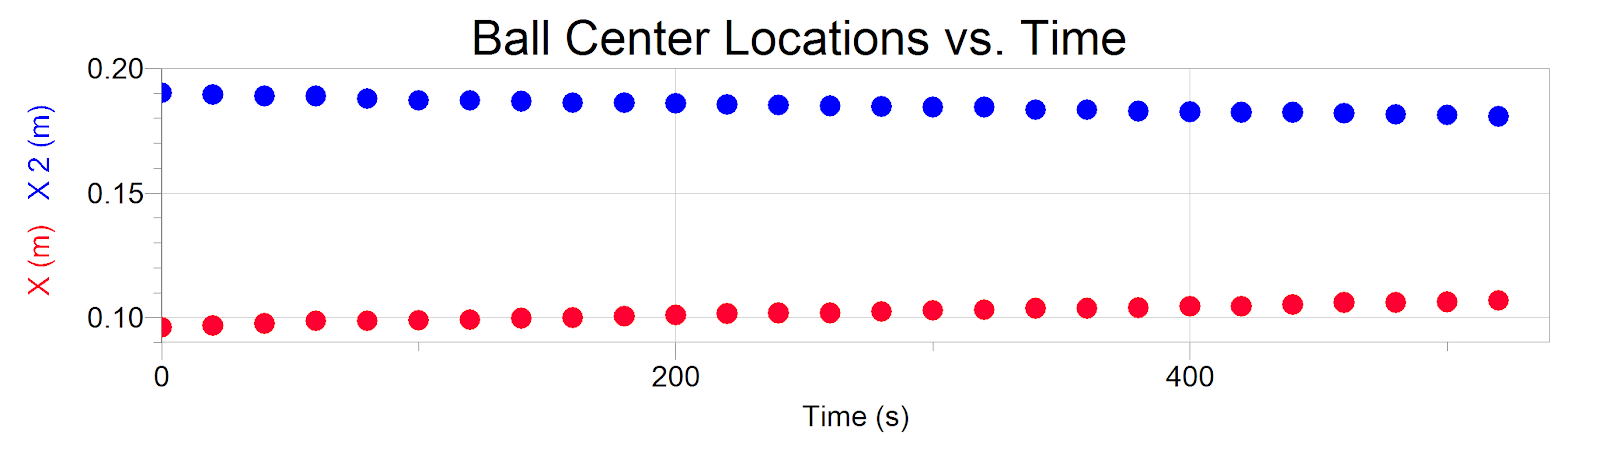
\includegraphics[width=\linewidth,scale=0.01]{LocvTime.png}
		%h (here) - same location
		%t (top) - top of page
		%b (bottom) - bottom of page
		%p (page) - on an extra page5
		%! (override) - will force the specified location
		\caption{The position of the center location of both ball 1 and ball 2, denoted as X (m) and X 2 (m) respectively, versus time (s).}
		\label{loc}
	\end{figure}
\begin{figure}[h]
	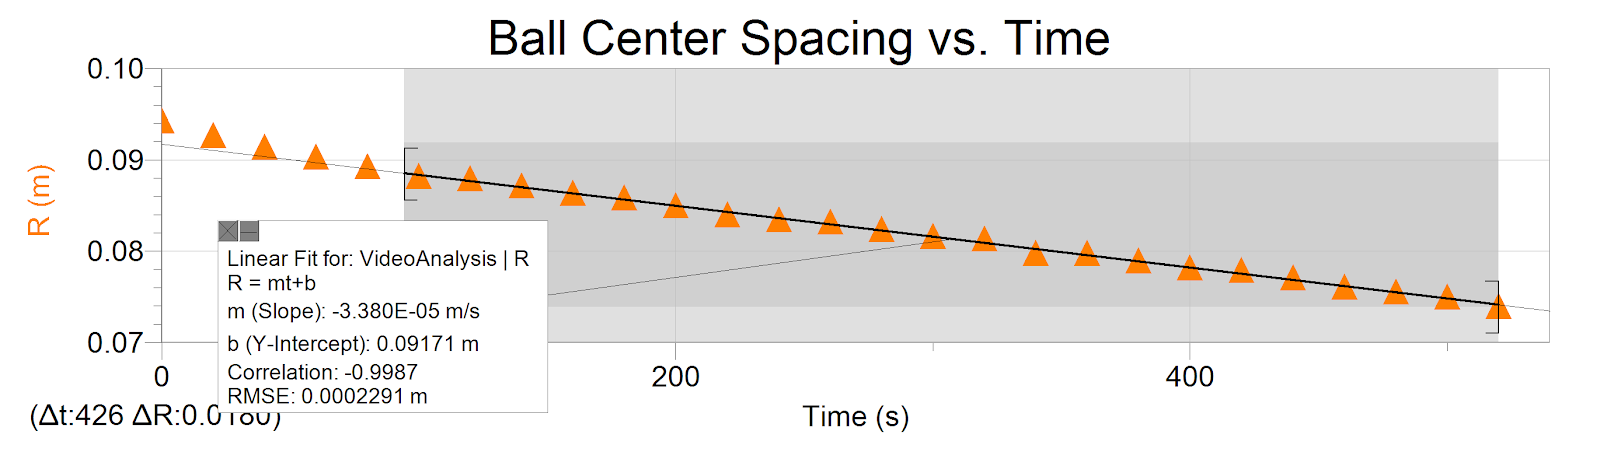
\includegraphics[width=\linewidth,scale=0.01]{SpacevTime.png}
	%h (here) - same location
	%t (top) - top of page
	%b (bottom) - bottom of page
	%p (page) - on an extra page5
	%! (override) - will force the specified location
	\caption{The separation of the centers of both ball 1 and ball 2, denoted as R (m), versus time (s).}
	\label{Space}
\end{figure}

\begin{figure}[h]
	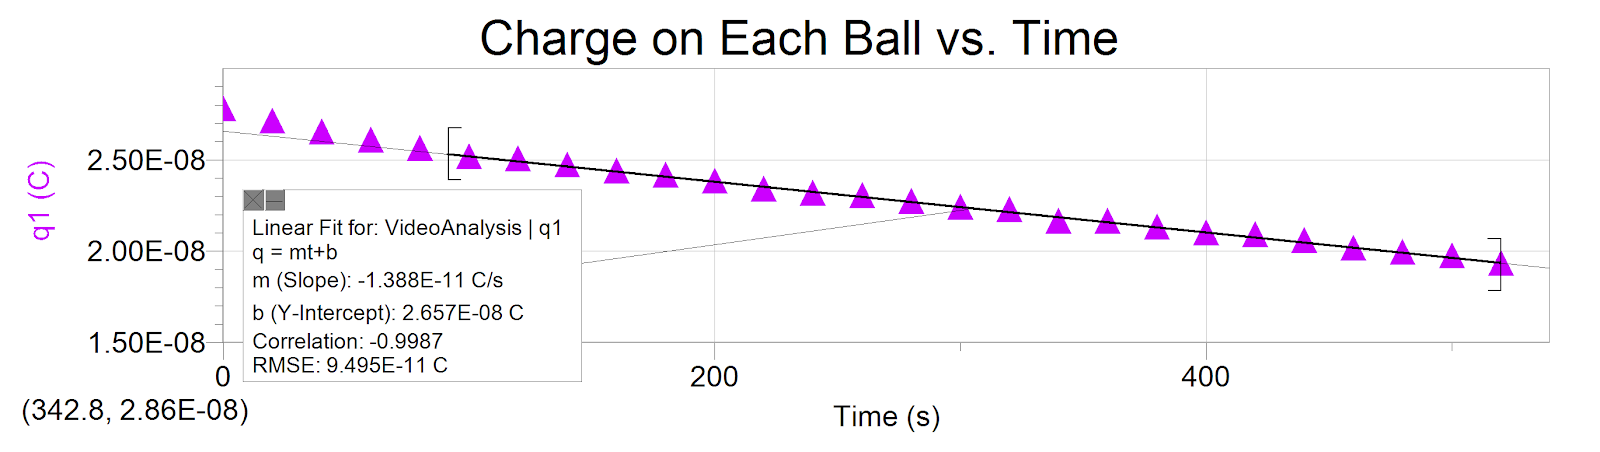
\includegraphics[width=\linewidth,scale=0.01]{ChargevTime.png}
	%h (here) - same location
	%t (top) - top of page
	%b (bottom) - bottom of page
	%p (page) - on an extra page5
	%! (override) - will force the specified location
	\caption{The charge on ball 1 (C) versus time (s). Given that the mass and charge of the two balls were nearly identical, only ball 1 was used for analysis.}
	\label{Charge}
\end{figure}
	
\end{document}